\chapter{Baryonic Structures}


\section{State and distribution of baryons}


We want to include baryons in the study of non-linear structure formation.

\subsection{Evolution}
Before recombination and decoupling, the baryons were an ionized plasma.

After recombination, they are mostly neutral and in atomic form. At that point, there is little emission, which is why this period is called the Dark Ages.

At later times ($z \approx 6$ -- $20$), the first stars start to form, which emit UV photons that re-ionize the baryons and end the Dark Ages. This is called the Epoch of Reionization (EoR).

Following this, the baryons continue to participate in structure formation, driven by dark matter.


\subsection{Phases}
\begin{itemize}
	\item Gas
	\begin{itemize}
		\item Hot gas (ionized)
		\item Cold gas (atomic or molecular form)
	\end{itemize}
	\item Stars
\end{itemize}
These different phases interact and convert to each other.


\subsection{Distribution}
\begin{itemize}
	\item within galaxies: Interstellar medium (ISM)
	\item between galaxies: Intergalactic medium (IGM)
	\item within galaxies clusters: Intra-cluster medium (ICM)
\end{itemize}



\subsection{Dynamics}
We know that there is five times as much dark matter mass as there is baryonic mass.
As a result, dark matter mostly drives the dynamics of structure formation and provides the backbone for the dynamics of the baryons.
Unlike dark matter, baryons are collisional, and their dynamics include various effects:
\begin{itemize}
	\item Thermodynamical effects: Heating and cooling
	\item Radiative transfer: Interaction between baryons and photons
	\item Hydrodynamical effects: Shocks
	\item Transitions between different phases: Star formation
	\item Astrophysical effects: Supernova explosions and active galactic nuclei
\end{itemize}
The dynamics of baryons is more complicated than that of dark matter.
Figure \ref{fig:illustris-evolution} shows the evolution of dark matter and ordinary matter from a simulation.

\begin{figure}
	\includegraphics[width=\textwidth]{img/ch-05/illustris-evolution.png}
	\caption{The evolution of dark matter and ordinary matter from the illustris simulation.}
	\label{fig:illustris-evolution}
\end{figure}

Generally, some baryons tend to sink to the bottom of potential wells, driven by dark matter on small scales, because baryons have dissipation.

Our approach here is to first review astrophyiscal facts about baryonic structures and discuss approaches for modelling the baryons.





\section{Stars}

Stars are formed by the collapse of cold gas in molecular clouds in the ISM.
They are supported against gravity by nuclear fusion reactions at their centre.
The energy that is produced is transported outwards by photons to the star's outer shells.

\subsection{Composition}
\begin{table}
	\begin{tabular}{lccccccccc}
	\toprule
	Element & H & He & C & N & O & Ne & Mg & Si & Fe\\
	\midrule
	$(N/N_H) \cdot 10^5$ & $10^5$ & 9800 & 36.3 & 11.2 & 85.1 & 12.3 & 3.80 & 3.55 & 4.68\\
	\bottomrule
	\end{tabular}
	\caption{The chemical composition of the sun.}
	\label{tab:solar-comp}
\end{table}
The solar composition is shown in \cref{tab:solar-comp}.
For comparison, the primordial abundance is about \SI{75}{\percent} hydrogen and \SI{25}{\percent} helium, with only traces of heavier elements.
Apparently, the abundance of helium and heavier elements in the sun is different from the primordial abundance.
This is because heavier elements are produced by nuclear reactions in stars.
To characterize these abundances, we define the \emph{metallicity} $z$, which is the mass faction of elements heavier than helium.
For the sun, $z_\sol \approx \SI{2}{\percent}$.

\subsection{Classification}
\begin{margintable}
	\begin{tabular}{ll}
		\toprule
		Class & $T$ [K]\\
		\midrule
		O & \num{28000}--\num{50000}\\
		B & \num{10000}--\num{28000}\\
		A & \num{7500}--\num{10000}\\
		F & \num{6000}--\num{7500}\\
		G & \num{5000}--\num{6000}\\
		K & \num{3500}--\num{5000}\\
		M & \num{2500}--\num{3500}\\
		\bottomrule
	\end{tabular}
	\caption{The spectral type as a function of temperature.}
	\label{tab:spectral-type}
\end{margintable}
The modern classification system for stars is the MK classification, which consists of a spectral classification and a luminosity classification.

The spectral classification is a single letter for rough classification, followed optionally by a single number for finer classification.
\Cref{tab:spectral-type} shows the temperature of stars with different spectral types.

\subsection{Hertzsprung-Russel diagram}

The Hertzsprung-Russell (HR) diagram in \cref{fig:hr-gaia} shows the relationship between surface temperature and luminosity of stars in our galaxy.

\begin{figure}
	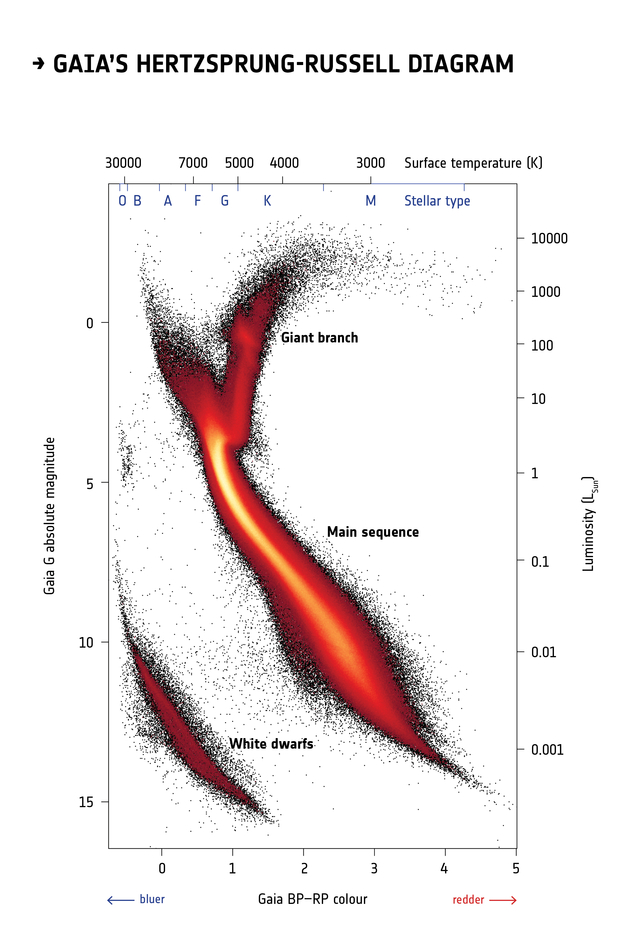
\includegraphics[width=\textwidth]{img/ch-05/hr-gaia.png}
	\caption{The Hertzsprung-Russell diagram, as measured by the GAIA satellite.}
	\label{fig:hr-gaia}
\end{figure}

The evolution of stars can be tracked on the HR diagram.
Stars are born on the main sequence (MS).
The phenomenological \emph{initial mass function} (IMF) is the distribution of newly born stars of the MS.
Eventually, they have burned all their hydrogen and start moving away from the MS towards the red giant branch (RGB).
Stars with higher masses exhaust their hydrogen first.
As a reg giant runs out of nuclear fuel, they collapse into compact objects. Depending on their mass, this compact object can be a white dwarf, a neutron star, or a black hole.
In the process, supernova explosions can be generated.
They inject kinetic energy into the ISM and disperse the heavy elements that the star generated.
This process is called enrichment of the ISM.

\subsection{Galaxies}
Galaxies contain many stars, so they can be used to track the stellar evolution.
Because the massive blue stars burn their fuel first, new galaxies are blue, and old galaxies are red.


\section{Classification of galaxies}

\begin{figure}
	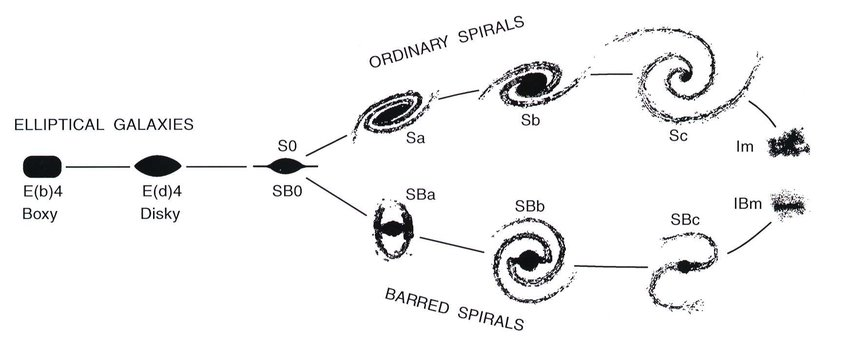
\includegraphics[width=\textwidth]{img/ch-05/tuning-fork.jpg}
	\caption{The Hubble tuning fork diagram classifies galaxies according to their shape.}
	\label{fig:tuning-fork}
\end{figure}

There is a wide range of types of galaxies.
A common classification is the Hubble sequence, also known as the tuning fork diagram, which is shown in \cref{fig:tuning-fork}.
The Hubble sequence distinguishes the following types:
\begin{itemize}
	\item Elliptical galaxies have a smooth elliptical light distribution. They are subdivided into E0 (spherical) to E7 (very flat).
	\item Spiral galaxies have a disk with spiral arms, and a central halo.
	\begin{itemize}
		\item Normal spiral galaxies go from Sa (tight spiral) to Sc (loose spiral).
		\item Barred spiral galaxies go from SBa (tight spiral) to SBc (loose spiral).
	\end{itemize}
	\item Lenticular galaxies (S0) are an intermediate step between ellipticals and spirals.
\end{itemize}
There are also other types of galaxies which are not on the Hubble sequence:
\begin{itemize}
	\item Irregular galaxies have irregular shapes.
	\item Peculiar galaxies have odd shapes and are often associated with mergers.
	\item Dwarf galaxies are galaxies with luminosities fainter than $M_B = -18$.
	\item Active galactic nuclei are very bright nuclei that can be found in some galaxies. They may be the only part of an otherwise faint galaxy that is visible to us.
\end{itemize}

Elliptical galaxies are called \enquote{early types}, and spirals are called \enquote{late types}.
The nomenclature is historical and is not related to the formation history.



% 5.4
\section{Elliptical galaxies}
Elliptical galaxies tend to be regular, with a smooth elliptical light distribution.

\subsection{Surface brightness}
The surface brightness of elliptical galaxies is well fit by a \emph{Sérsic profile},
\begin{align*}
	I(R)
	&= I_0 \exp\Bigg[ - \beta_n \left( \frac{R}{R_e}  \right)^{1/n} \Bigg],
\end{align*}
where $m$ is the Sérsic index,
$R$ is the semi-major axis length,
$R_e$ is the half-light radius,
and it follows that $\beta_n \approx 2 n - 0.324$ to fulfill this criterion.
The brighter galaxies have a larger value of $n$.
For normal ellipticals, $n \approx 4$, for which the profile is also called a \emph{de Vaucouleurs profile}.

\subsection{Shape}
Let $b/a$ be the ratio of minor to major axis of the light distribution.
For normal ellipticals, $b/a \in [0.3, 1]$.
In the Hubble sequence, this corresponds to types E0 to E7.

\subsection{Colour}
Ellipticals tend to be redder than spirals, which indicates an older, metal-rich star population.
Some ellipticals have colour gradients, such that the central regions tend to be redder.

\subsection{Kinematics}
The support against gravitational collapse is mostly provided by random motion.
The rotational velocities are comparatively small.


\subsection{Scaling relations}
\begin{figure}
	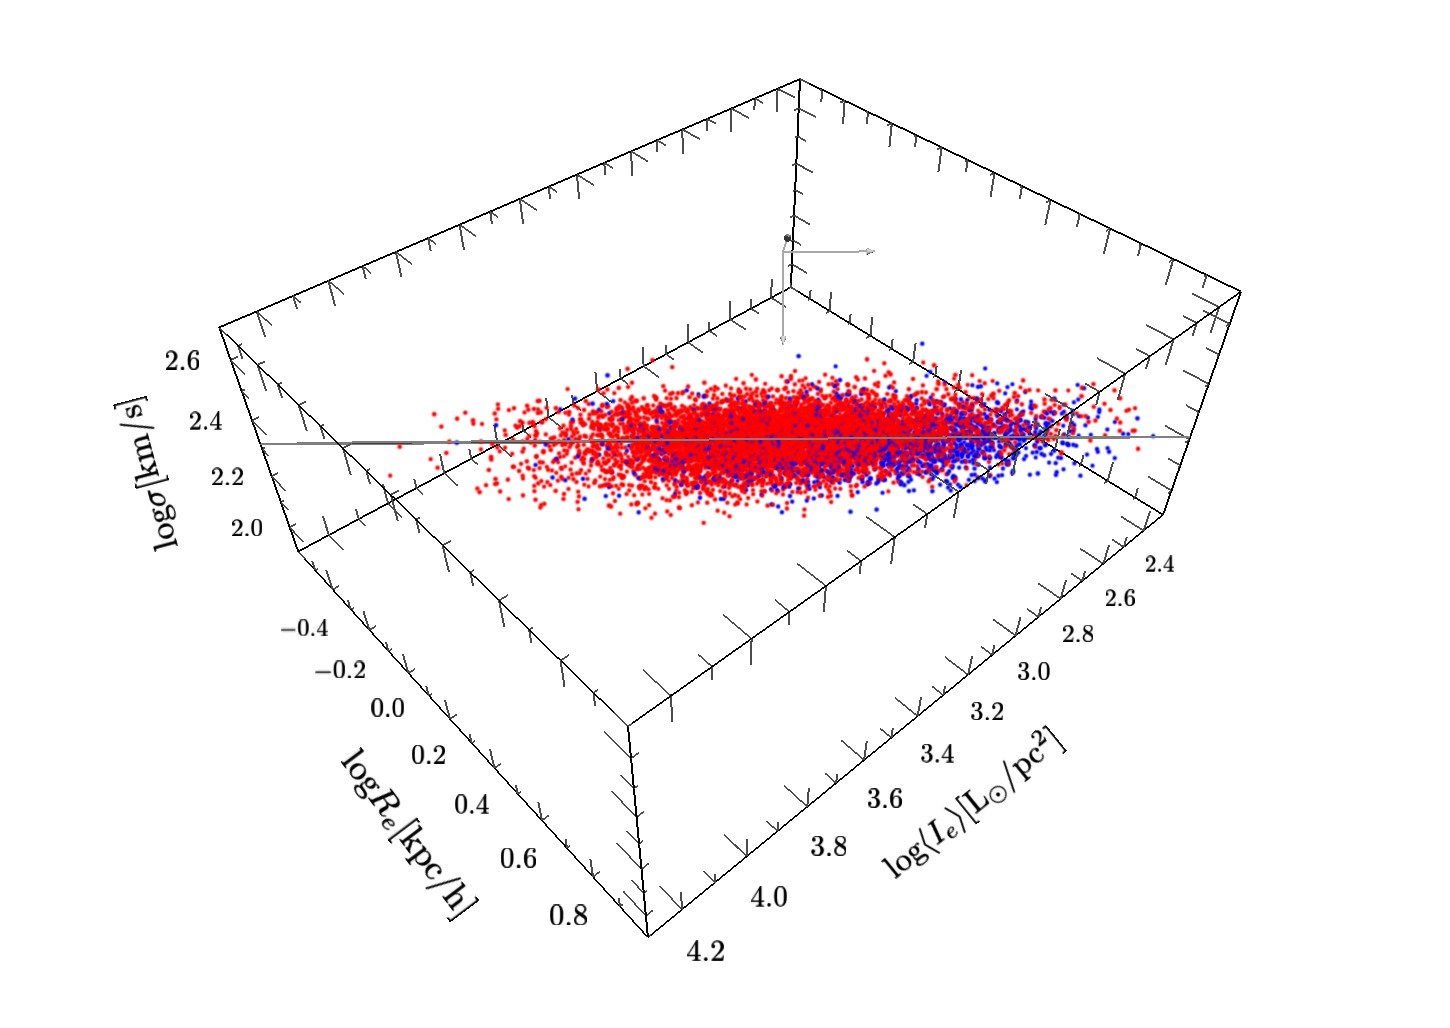
\includegraphics[width=0.7\textwidth]{img/ch-05/fundamental-plane.png}
	\caption{The fundamental plane for elliptical galaxies. The view is chosen such that the plane is seen edge-on as a line.}
	\label{fig:fundamental-plane}
\end{figure}
There is a correlation between some of the main characteristics of ellipticals.
Let $\sigma$ be the line of sight velocity dispersion of stars inside the half-light radius $R_e$,
and let $\avg{I}_l$ be the main surface brightness within $R_e$.
\Cref{fig:fundamental-plane} shows the \emph{fundamental plane}, which which quantifies the correlation between these parameters.
% \sidecite{Magoulas:2012jy}
% TODO
The correlation between $\avg{I_l}$ and $\sigma$ is called \emph{Faber-Jackson relation}.
The correlation between $R_e$ and $\sigma$ is called the \emph{$D_n$-$\sigma$ relation}, whose name comes from an other measure for radius, $D_n$.


\subsection{Gas content}
Very little cold gas, with temperatures less than \SI{100}{\kelvin}, is contained in ellipticals.
As a result, new stars are not forming, which explains the old stellar population.
Hot gas with temperatures around \SI{e7}{\kelvin} is much more abundant, and can be found with x-ray observations.
There is also a little warm gas, with temperature \SI{e4}{\kelvin}.







\section{Spiral galaxies}
\begin{marginfigure}
	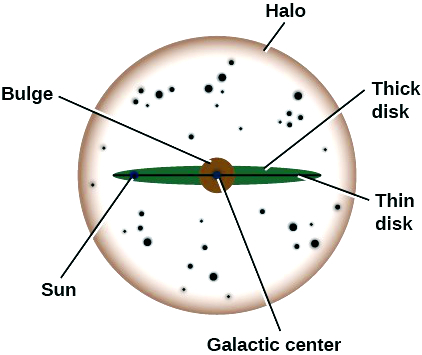
\includegraphics[width=\textwidth]{img/ch-05/milky-way.png}
	\caption{Structure of the Milky Way.}
	\label{fig:mw-structure}
\end{marginfigure}
Spiral galaxies, like the Milky Way in \cref{fig:mw-structure}, show a spiral structure when viewed face-on, and look like a flat disk with a central bulge edge-on.
They also have a dark matter halo, which surrounds and includes the visible structure.

\subsection{Surface brightness}
The disks of spiral galaxies are well fitted by an exponential profile,
\begin{align*}
	I(R)
	&= I_0 \exp\left( -\frac{R}{R_d} \right),
\end{align*}
which is a Sérsic profile with Sérsic index $n=1$,
and $R_e \approx 1.67 R_d$.
More luminous spirals usually have larger radii.
Bulges are also well fitted by a Sérsic profile, with $n = 4$ for large bulges, down to $n=1$ for smaller ones.

\subsection{Colour}
Spirals tend to be blue, which indicates a younger and still forming stellar population in the disk.
More luminous disks tend to be redder.
The star formation rate $\dot{M}_* = \dv{M_*}{t}$, where $M_*$ is the total mass of stars in a galaxy, varies considerably between galaxies.
Galaxies with very high star formation rates are called \emph{Starburst galaxies}.

The stellar haloes are mostly made up of old metal-poor stars.
More than half of all spiral galaxies have a bar.
The spiral arms are typically bluer and contain regions of star formation.

\subsection{Gas content}
Spirals have mostly cold gas in the disk, which gives them a reservoir for star formation.

\subsection{Kinematics}
\begin{marginfigure}
	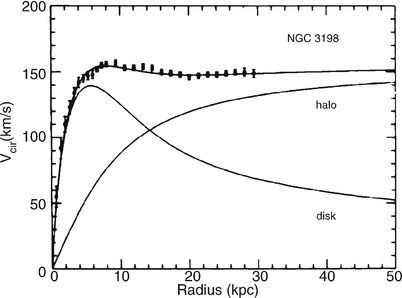
\includegraphics[width=\textwidth]{img/ch-05/rotation-curve.png}
	\caption{The rotation curve of the galaxy NGC 3198. The rotation curve is the result of a contribution from baryonic matter in the disk and a dark matter halo, which extends beyond the disk. The baryonic matter is on average closer to the centre of the galaxy, because unlike dark matter, it can lose energy by dissipation.}
	\label{fig:rotation-curve}
\end{marginfigure}
The disks in spirals are rotationally supported, with approximately circular orbits for stars and gas.
According to Newtonian gravity, the rotational velocity $v_\text{rot}$ of a star at radius $r$ can be found as follows:
\begin{alignat*}{3}
	         && F &= ma\\
	&\implies & \frac{G m M(r)}{r^2} &= m \frac{v_\text{rot}^2}{r}\\
	&\implies & v_\text{rot} &= \sqrt{\frac{G M(r)}{r}}.
\end{alignat*}
\Cref{fig:rotation-curve} is the rotation curve of the galaxy NGC 3198, which shows that the rotational velocity as a function of radius rises quickly and then remains flat, which cannot be explained from the visible matter alone, since we would expect a fall-off of the rotational velocity along with the brightness profile.
Apparently, there must be another invisible contribution to the mass, which comes from the dark matter halo.
For $v_\text{rot}$ to be constant, we need $M(r) \propto r$, which implies $\rho(r) \propto r^{-2}$.
The NFW profile at intermediate radii is a good model for this.

\subsection{Scaling relations}
The correlation between the maximal rotational velocity $v_\text{max}$ and the luminosity $L$ is well fitted by
\begin{align*}
	L = A v_\text{max}^\alpha, 
	\qquad \text{with } \alpha \in [2.5, 4],
\end{align*}
which is called the \emph{Tully-Fisher relation}.




\section{Dwarf galaxies}
Dwarf galaxies are galaxies with low luminosities, such that $M_B \geq - 18$.
\Cref{fig:dwarfs} shows that they can have diverse structures, and they can be separated into different subtypes.
\begin{itemize}
	\item Dwarf galaxies that are gas rich, show strong star formation, and have irregular shapes are called \emph{Dwarf irregulars}, dIrr.
	\item Dwarf galaxies that are gas poor, without young stars, and with regular structures, are subdivided into \emph{Dwarf ellipticals}, dE, and the fainter Dwarf spheroidals, dSph.
\end{itemize}


\section{Active galactic nuclei}
\emph{Active galactic nuclei} (AGN) are very luminous centres that can be found in some galaxies, which are then called \emph{active galaxies}.
Observationally, they come in different subclasses, some of them being Seyfert galaxies, quasars, blazars, radio AGN, and liners.

AGNs have spectra that are very different from what one would expect from stellar sources, since they emit strongly across the entire range of the electromagnetic spectrum, from the radio to the gamma ray range, and they contain strong emission lines.

The emission is variable on a time scale of a few days, so for the emission region to be causally connected, it must be smaller than a few light days.
This is a very compact length scale compared to the rest of the galaxy.

AGNs are powered by accretion onto a supermassive black hole (\textsc{smbh}), with masses around \SIrange{e6}{e9}{\solarmass}.
The \textsc{smbh} grows as it accretes gas, and it can also reinject energy into the \textsc{igm} in the form of jets.
Accretion can be a very efficient process to convert gravitational energy into radiation.
While most galaxies, including the Milky Way, have an \textsc{smbh} in their centre, they are not necessarily \emph{active} galaxies.

The wide range of types of AGNs can be squeezed reasonably well into unification models, which state that they are all roughly similar kinds of objects, but observed from different viewing angles.

\section{Statistical properties of the galaxy population}

\subsection{Luminosity function}
The luminosity function $\phi(L) \dd{L}$ is defined as the number density of galaxies with luminosities between $L$ and $L + \dd{L}$.
For a wide range of galaxies, a \emph{Schechter function} is a good fit:
\begin{align*}
	\phi(L) \dd{L}
	&= \phi^* \left( \frac{L}{L^*} \right)^\alpha
	\exp\left( - \frac{L}{L^*} \right)
	\frac{\dd{L}}{L^*},
\end{align*}
where
$L^*$ is a characteristic luminosity,
$\alpha$ is the faint end slope,
and $\phi^*$ is a normalization factor.
% TODO figure
In \cref{fig:lum-func}, the luminosity function has been fitted to experimental data.

\subsection{Colour distribution}
\begin{marginfigure}
	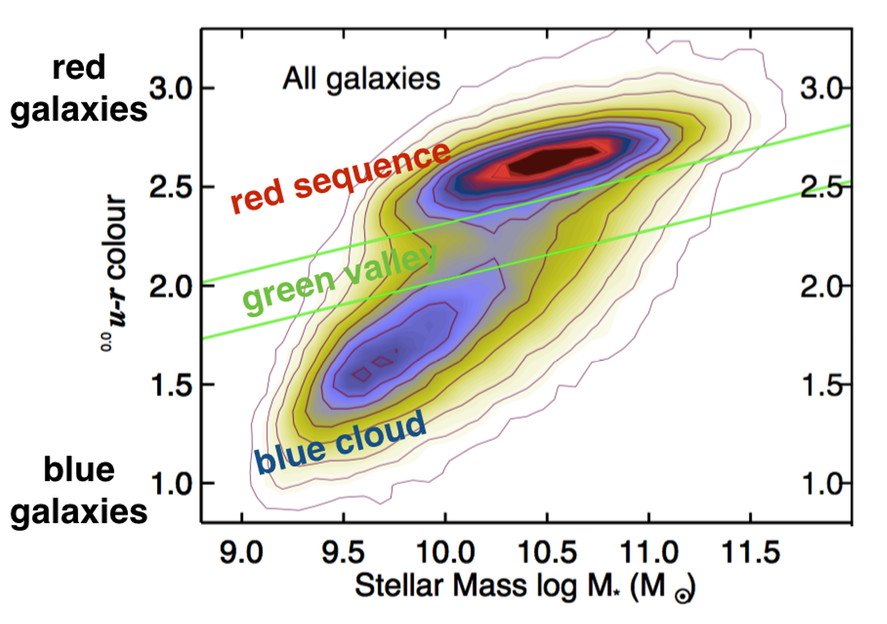
\includegraphics[width=\textwidth]{img/ch-05/cm-galaxies.png}
	\caption{The color-mass diagram for galaxies.}
	\label{fig:cm-galaxies}
\end{marginfigure}
The color-mass diagram for galaxies is shown in \cref{fig:cm-galaxies}.
There are two maxima in the distribution: 
The red sequence consists of bright red galaxies,
and the blue cloud consists of faint blue galaxies.

\subsection{Mass-Metalicity}
Spiral galaxies with large total stellar masses $M_*$ tend to have higher metalicities.

\subsection{Clustering}
Galaxies in denser regions are redder.
Equivalently, elliptical galaxies are more clustered than spiral galaxies.
% TODO figure
The fraction of different kinds of galaxies is shown as a function of density.







\section{Clusters and groups of galaxies}

\subsection{Clusters of galaxies}
Galaxy clusters are the largest bound objects in the universe.
\begin{itemize}
	\item Number of galaxies: 50 to a few thousand
	\item Radius: a few \si{\mega\parsec}
	\item Mass: \SIrange{e14}{e15}{\solarmass}
	\item Velocity dispersion (line of sight): $\sigma_\text{los} \approx \SI{1000}{\kilo\metre\per\second}$
\end{itemize}

Criteria for selecting clusters:
\begin{itemize}
	\item Richness: The number of galaxy members
	\item Compactness: Number of galaxies within a given radius
	\item Regularity: Circularity or smoothness
\end{itemize}

An example of a survey is the Abell cluster catalogue from 1958.

Nearby clusters are Virgo and Coma.

\paragraph*{Galaxy population}
Clusters are rich in early type (red, elliptical) galaxies.
For regular clusters, \SI{80}{\percent} of galaxies are E or S0, which is higher than the average in the field (outside clusters), about \SI{30}{\percent}.

The fraction of red galaxies tends to decrease in clusters with increasing redshift, which is known as the \emph{Butcher-Oemler effect}.

The radial density of galaxies in clusters is similar to the distribution of dark matter, which indicates that the galaxies act as collisionless particles.

Often, the brightest galaxy in a cluster is very extended, diffuse, and near the centre. They are called cD galaxies, and are thought to have grown through the accretion of multiple galaxies.
The effect is called \emph{galaxy cannibalism}.

\paragraph*{Mass estimation}
There are several techniques to measure the mass of a cluster:
\begin{itemize}
	\item \textbf{Velocity dispersion:}
	Along the line of sight, a velocity dispersion of $\sigma_\text{los} \approx \SI{1000}{\kilo\metre\per\second}$ can be measured with redshift.
	The Virial theorem then yields
	\begin{align*}
		M \approx A \frac{\sigma_\text{los}^2 R}{G},
	\end{align*}
	where the constant $A$ depends on the profile of the cluster and the exact definition of the radius $R$.
	\item \textbf{X-ray emission:}
	The hot gas ($T \approx \SI{e7}{\kelvin}$) in the intra-cluster medium emits bremsstrahlung, which is in the X-ray range.
	If we assume hydrostatic equilibrium, such that the gas is in equilibrium with the gravitational potential, then the X-ray emission profile and the X-ray temperature can be used to derive the total mass of the cluster and the gas.
	\item \textbf{Gravitational lensing:}
	A cluster of galaxies can act as a gravitational lens for the background galaxies.
	The trajectories of photons from distant objects are deflected by the gravitational potential of a cluster.
	The mass of the cluster can be derived from the strength of distortion of the background galaxies.
\end{itemize}

One finds that the mass of clusters is in the range \SIrange{e14}{e15}{\solarmass}.
Also, only \SI{10}{\percent} of the mass is baryonic in nature, which is strong evidence for the existence of dark matter.





\subsection{Groups of galaxies}
\begin{itemize}
	\item Number of galaxies: 3 to 30
	\item Radius: \SIrange{0.1}{1}{\mega\parsec}
	\item Mass: \SIrange{e12.5}{e14}{\solarmass}
	\item Velocity dispersion: $\sigma_\text{los} \approx \SI{300}{\kilo\metre\per\second}$
\end{itemize}

An example is the local group, with its largest member, the Milky Way.
There are many Milky Way satellites, such as the small Magellanic cloud (\textsc{smc}) and the large Magellanic cloud (LMC).
Another large galaxy in the local groups is the Andromeda galaxy (M31).






\section{Intergalactic medium}

The intergalactic medium (IGM) is made up of the baryons between galaxies.
It is usually too diffuse and not hot enough to be studied in emission,
but it can be seen in absorption.

\paragraph*{Quasar absorption lines}
% TODO diagram quasar
Suppose a distant quasar is at redshift $z_q$, and clouds of IGM are in front of it at different redshifts $z_i$, with $i = 1, 2, 3, \dots$.
The continuum light of the quasar is absorbed by the clouds, particularly by the strong Lyman-alpha transition, with (rest) wavelength $\lambda_\mathrm{α} = \SI{1216}{\angstrom}$.
We thus see absorption lines at wavelengths $\lambda_\mathrm{α} (1 + z_i)$.
% TODO spectrum quasar

The central peak is the Ly-α emission of the quasar itself, which is redshifted to around \SI{5400}{\angstrom}, indicating $z_q \approx 3.5$.
On the left side, there are many absorption lines, corresponding to Ly-α absorption at different redshifts.
There are also a few absorption lines on the right from metals.

We distinguish different types of absorption systems:
\begin{itemize}
	\item The \textbf{Ly-α forest} consists of many thin absorption lines,
	corresponding to a column density of neutral hydrogen $N_{\mathrm{H}\textsc{i}} \leq \SI{e17}{\centi\meter\tothe{-2}}$.
	\item \textbf{Damped Ly-α systems} have larger column densities of $N_{\mathrm{H}\textsc{i}} \geq \SI{e20}{\centi\meter\tothe{-2}}$,
	which absorb the quasar light completely at the Ly-α wavelength.
\end{itemize}












